\chapter{NumPy, Matplotlib e Pandas}\label{numpy}

A lista (\inlcode{list}) em Python é uma estrutura de dados altamente versátil: cada elemento pode conter qualquer tipo
de objeto, independentemente do tamanho ou tipo, e a estrutura pode ser modificada e redimensionada dinamicamente.
No entanto, toda essa generalidade e flexibilidade tem um custo, especialmente em termos de desempenho.

Diferente de outras linguagens, o Python não possui um tipo embutido para representar \inlcode{arrays} no sentido
tradicional, ou seja, coleções de dados homogêneos com tamanho fixo.
Esse tipo de estrutura, embora bem mais restrita que uma lista, permite otimizações tanto no uso de memória quanto
na performance.

Isso torna-se particularmente crítico quando lidamos com grandes volumes de dados numéricos em aplicações
científicas, como regressão, otimização, álgebra linear os demais métodos utilizados em
computação científica.
Nessas situações, a eficiência no processamento é essencial, exigindo estruturas de dados mais especializadas e
performáticas que as listas tradicionais do Python.

A solução mais amplamente adotada para esse desafio em Python é o uso da biblioteca \inlcode{numpy}, que, embora não
venha incluída por padrão na instalação da linguagem, consolidou-se como o padrão de fato no meio científico para
computação numérica.
Complementarmente, as bibliotecas \inlcode{pandas} e \inlcode{matplotlib} são amplamente utilizadas, respectivamente,
para a manipulação e análise de dados estruturados (como tabelas), bem como para a visualização de dados por meio da
geração de gráficos (\inlcode{plots}).

Como \inlcode{numpy}, \inlcode{matplotlib} e \inlcode{pandas} não fazem parte da biblioteca padrão, é necessário
instalá-los manualmente.
Isso pode ser feito utilizando o \inlcode{pip}, o gerenciador de pacotes oficial do Python.
Para realizar a instalação, basta executar o seguinte comando no terminal:
\begin{minted}[escapeinside=??]{text}
?\textcolor{green!20!brown}{C:\char92curso\_python\char92>}? pip install numpy matplotlib pandas
\end{minted}


\section{NumPy}

A biblioteca \inlcode{numpy} fornece a estrutura de dados \inlcode{ndarray}, que permite representar
\inlcode{arrays} multidimensionais de forma compacta e eficiente.
Ela também disponibiliza um vasto conjunto de funções vetorizadas otimizadas, capazes de aplicar operações matemáticas
diretamente sobre todo o \inlcode{array}, dispensando o uso de laços explícitos que podem ser pouco performáticos em Python.
Essa abordagem vetorizada resulta em cálculos muito mais rápidos, especialmente ao lidar com grandes volumes de dados.

Uma das aplicações fundamentais da \inlcode{numpy} é na representação e manipulação de matrizes.
O exemplo a seguir ilustra esse uso:
\begin{minted}[linenos]{custompython}
import numpy as np

A = np.array([[2, 3],    # define matriz 2 x 2
              [-4, 1]])
x = np.array([[3],       # define matrix 2 x 1
              [1]])
b = np.array([[-3],      # define matrix 2 x 2
              [8]])

y = A @ x + b    # operação de multiplicação e soma matricial
print(y)
\end{minted}
\begin{minted}{text}
[[ 6]
 [-3]]
\end{minted}

Na \textbf{linha 1}, declaramos que utilizaremos o pacote \inlcode{numpy}, e o faremos por meio do \emph{alias}
\inlcode{np}.
Ou seja, para não repetirmos \inlcode{numpy} diversas vezes ao longo do código, atribuímos a ele o nome
abreviado \inlcode{np}.

Na \textbf{linha 3}, criamos a matriz $\mathbf{A}$ de dimensão $2 \times 2$ utilizando \inlcode{array}.
Já nas \textbf{linhas 5} e \textbf{7}, definimos os vetores coluna $\mathbf{x}$ e $\mathbf{b}$,
ambos com dimensão $2 \times 1$.


E na \textbf{linha 10} realizamos a operação matricial $\mathbf{y} = \mathbf{A} \cdot \mathbf{x} + \mathbf{b}$.
Observe que o operador \inlcode{@} realiza o produto matricial, conforme definido na álgebra linear.
Já o operador \inlcode{*} também pode ser utilizado com arrays \inlcode{numpy}, mas nesse caso representa
a multiplicação elemento a elemento, e não a multiplicação de matrizes.

Por fim, na \textbf{linha 10}, realizamos a operação matricial $\mathbf{y} = \mathbf{A} \cdot \mathbf{x} + \mathbf{b}$.
Note que o operador \inlcode{@} realiza o produto matricial, conforme definido na álgebra linear.
Já o operador \inlcode{*} também pode ser usado com \inlcode{arrays} do \inlcode{numpy},
mas nesse caso ele representa a multiplicação elemento a elemento, e não o produto de matrizes.

Além das operações matriciais, o \inlcode{numpy} também se destaca ao lidar com sequências numéricas unidimensionais,
graças à sua poderosa implementação de vetorização --- que simplifica tanto a escrita do código quanto sua performance.

No exemplo a seguir, usamos um \inlcode{array} para representar uma sequência numérica e, com isso, podemos usar
vetorização para aplicar uma expressão matemática a cada elemento dessa sequência:
\begin{minted}[linenos]{custompython}
import numpy as np

x = np.linspace(0, 3, 7)
y = x**2 - 2*x

print(f"{x = }")
print(f"{y = }")
\end{minted}
\begin{minted}{text}
x = array([0. , 0.5, 1. , 1.5, 2. , 2.5, 3. ])
y = array([ 0.  , -0.75, -1.  , -0.75,  0.  ,  1.25,  3.  ])
\end{minted}

Na \textbf{linha 3}, utilizamos o método \inlcode{linspace} da biblioteca \inlcode{numpy} para criar um \inlcode{array}
unidimensional (um vetor linha) contendo \inlcode{7} valores do tipo \inlcode{float}, igualmente espaçados no intervalo fechado de \inlcode{0} a
\inlcode{3} --- ou seja, incluindo os dois extremos do intervalo.

Na \textbf{linha 4}, exploramos as funcionalidades de vetorização da biblioteca \inlcode{numpy} para aplicar a
expressão matemática diretamente a todos os elementos de \inlcode{x}.
O resultado é um novo \inlcode{array y}, de mesmo tamanho, cujos valores correspondem à aplicação da expressão
$y_n = x_n^2 - 2x_n$ em cada elemento $x_n$ do \inlcode{array x}, sem a necessidade de laços explícitos.

Nos exemplos anteriores, usamos \inlcode{np.array([...])} para criar um \inlcode{array} a partir de uma
lista e \inlcode{np.linspace()} para gerar valores igualmente espaçados dentro de um intervalo.
Além dessas abordagens, a biblioteca \inlcode{numpy} oferece outras funções bastante úteis para a criação de
\inlcode{arrays}, como:
\begin{itemize}
\item [] \inlcode{np.zeros(shape)} -- cria um \inlcode{array} preenchido com zeros.
\item [] \inlcode{np.ones(shape)} -- cria um \inlcode{array} preenchido com uns.
\item [] \inlcode{np.full(shape, valor)} -- cria um \inlcode{array} preenchido com um valor específico.
\item [] \inlcode{np.eye(n)} -- gera a \inlcode{matriz} identidade de ordem \inlcode{n}.
\item [] \inlcode{np.arange(início, fim, passo)} -- semelhante à função \inlcode{range}, mas para \inlcode{array}.
\item [] \inlcode{np.random.rand(shape)} -- cria um \inlcode{array} com valores aleatórios no intervalo \inlcode{[0, 1)}.
\end{itemize}

Os exemplos apresentados acima têm como objetivo apenas introduzir a \inlcode{numpy}.
Ela oferece uma ampla gama de funcionalidades não abordadas, incluindo muitas outras operações vetoriais, manipulação
de arrays multidimensionais, transformações estruturais, mapeamento e interpolação de valores, entre muitos outros
recursos voltados à computação numérica.
Recomenda-se que o leitor explore essas funcionalidades conforme sua necessidade.
A documentação oficial da biblioteca está disponível em: \colorurl{https://numpy.org/doc}.


Além disso, recomenda-se ao leitor explorar a biblioteca \inlcode{SciPy}, que complementa e expande as funcionalidades
do \inlcode{numpy} ao disponibilizar ferramentas especializadas para áreas como álgebra linear, equações diferenciais,
integração numérica, otimização, interpolação, transformadas e processamento de sinais.
A documentação oficial da biblioteca está disponível em: \colorurl{https://docs.scipy.org/doc/scipy/}.


\section{Matplotlib}

Outra biblioteca particularmente útil em aplicações de computação científica é a \inlcode{matplotlib}.
Com uma pequena modificação no exemplo anterior, podemos utilizá-la para gerar um gráfico que representa
\inlcode{x} e \inlcode{y} no plano cartesiano.
\begin{minted}{custompython}
import numpy as np
import matplotlib.pyplot as plt

# gera valores para os eixos x e y do gráfico
x = np.linspace(0, 3, 100)
y = x**2 - 2*x

# plota o gráfico
plt.plot(x,y)
plt.show()
\end{minted}

Esse código gera e exibe a figura:
\begin{center}
    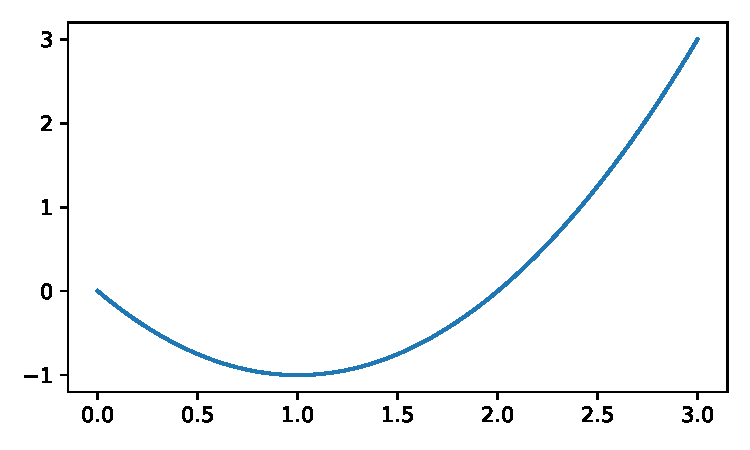
\includegraphics[scale=1.0]{figs/parabola}
\end{center}

A figura gerada exibe o gráfico construído a partir dos pares ordenados $(x_n, y_n)$.
Embora seja uma visualização simples, a biblioteca \inlcode{matplotlib} oferece uma ampla variedade
de funções auxiliares para personalizar o aspecto visual do gráfico.

O exemplo a seguir demostra algumas dessas funcionalidades:
\begin{minted}[linenos]{custompython}
import numpy as np
import matplotlib.pyplot as plt

# gera pontos para os eixo x e y
theta = np.linspace(0, 3*np.pi, 100)
y1 = np.sin(theta)
y2 = 0.7 * np.sin(theta - np.pi/3)
y3 = y1 + y2

# descomete caso queira fidelidade de fontes com Latex (necessário instalar Latex)
#plt.rcParams.update({'text.usetex': True, 'font.family': 'serif'})

plt.figure(figsize=(5, 2.8))    # define o latgura e altura da figura em polegadas
plt.plot(theta, y1, color='olivedrab' , linestyle='-.', label=r'$y_1$')     # plota y1
plt.plot(theta, y2, color='steelblue' , linestyle='--', label=r'$y_2$')     # plota y2
plt.plot(theta, y3, color='darkorange', linewidth=1.8 , label=r'$y_1+y_2$') # plota y3
plt.title('Gráfico de Exemplo')       # adiciona título ao gráfico
plt.xlabel(r'$\theta$ [rad]')         # adiciona identificação do eixo x
plt.ylabel(r'$y(\theta)$')            # adiciona identificação do eixo y
plt.xlim(theta[0], theta[-1])         # define os limites do eixo x
plt.ylim(1.2*y3.min(), 1.2*y3.max())  # define os limites do eixo y
plt.grid(True)       # exibe grade
plt.legend()         # exibe legenda (valores atribuidos a plabel no plot)
plt.tight_layout()   # ajusta o grafico gerado aos limites da figura

# define os ticks do eixo x manualmente como múltiplos de π
xticks = [0, np.pi/2, np.pi, 3*np.pi/2, 2*np.pi, 5*np.pi/2, 3*np.pi]
xtick_labels = [r'0', r'$\frac{\pi}{2}$', r'$\pi$', r'$\frac{3\pi}{2}$',
                r'$2\pi$', r'$\frac{5\pi}{2}$', r'$3\pi$']
plt.xticks(xticks, xtick_labels)

# exporta a figura gerada para um arquivo externo do tipo .pdf
plt.savefig(r"seno.pdf", format="pdf")

# exibe a figura na tela
plt.show()
\end{minted}

Saída do programa:
\begin{center}
    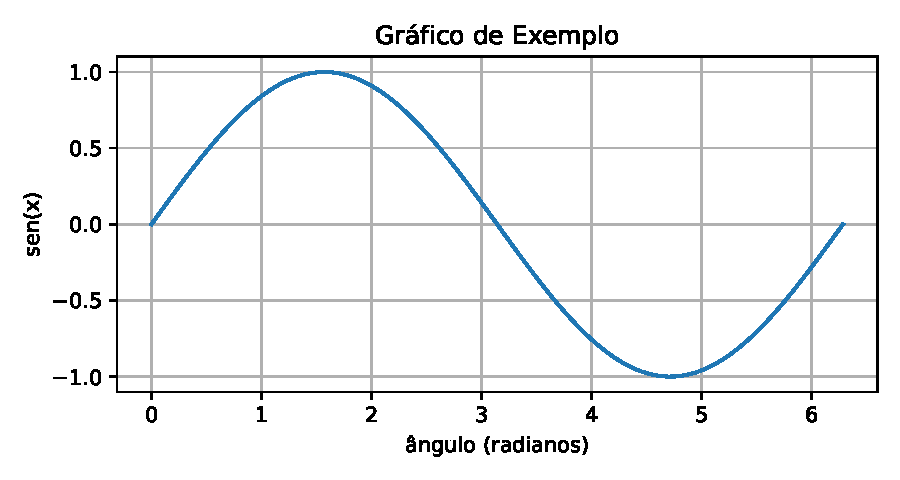
\includegraphics[scale=1.0]{figs/seno}
\end{center}

Mais informações sobre os recursos de \inlcode{matplotlib} podem ser encontradas na documentação oficial da biblioteca,
disponível em: \colorurl{https://matplotlib.org/stable/contents.html}.



\section{Pandas}

Assim como a biblioteca \inlcode{numpy} fornece uma estrutura para representar \inlcode{arrays} de elementos homogêneos,
a biblioteca \inlcode{pandas} introduz a estrutura \inlcode{DataFrame}, destinada a representar e manipular tabelas.

Um \inlcode{pandas.DataFrame} é, de forma simplificada, uma tabela com linhas e colunas rotuladas, semelhante a uma
planilha do \inlcode{Excel}.

Veja um exemplo simples:
\begin{minted}{custompython}
import pandas as pd

df = pd.DataFrame(data={'nome': ['Fulano', 'Beltrano', 'Sicrano'],
                        'documento': [5342, 1876, 1872],
                        'idade': [25, 15, 43],
                        'habilitado': [False, False, True],
                        })

print(df)
\end{minted}
\begin{minted}{text}
       nome  documento  idade  habilitado
0    Fulano       5342     25       False
1  Beltrano       1876     15       False
2   Sicrano       1872     43        True
\end{minted}

Neste exemplo, \inlstr{nome}, \inlstr{documento}, \inlstr{idade} e \inlstr{habilitado} são os rótulos das colunas,
que podemos utilizar para acessar, filtrar ou manipular os dados armazenados no \inlcode{DataFrame}.

Por exemplo, se quisermos acessar toda a coluna \inlstr{idade} para calcular a idade média dos usuários cadastrados,
podemos faze-lo com:
\begin{minted}{custompython}
idade_media = df['idade'].mean()
print(f'idade média: {idade_media:.1f} anos')
\end{minted}
\begin{minted}{text}
idade média: 27.7 anos
\end{minted}

Ou ainda, se desejarmos filtrar apenas os usuários não habilitados:
\begin{minted}{custompython}
nao_habilitados = df[df['habilitado'] == False]
print(nao_habilitados)
\end{minted}
\begin{minted}{text}
       nome  documento  idade  habilitado
0    Fulano       5342     25       False
1  Beltrano       1876     15       False
\end{minted}

Ou apenas os maiores de idade:
\begin{minted}{custompython}
maiores_idade = df[df['idade'] >= 18]
print(maiores_idade)
\end{minted}
\begin{minted}{text}
      nome  documento  idade  habilitado
0   Fulano       5342     25       False
2  Sicrano       1872     43        True
\end{minted}

Ou se desejarmos, naão filtrar, mas ordenar pela idade:
\begin{minted}{custompython}
df_ordenado = df.sort_values(by='idade')
print(df_ordenado)
\end{minted}
\begin{minted}{text}
       nome  documento  idade  habilitado
1  Beltrano       1876     15       False
0    Fulano       5342     25       False
2   Sicrano       1872     43        True
\end{minted}

As possibilidades são inúmeras.
A biblioteca provê meios de acessar, filtrar, manipular e transformar dados de forma
expressiva e eficiente — tudo com poucas linhas de código.

Note ainda que, neste exemplo introdutório, definimos explicitamente quatro colunas (\inlstr{nome}, \inlstr{documento},
\inlstr{idade} e \inlstr{habilitado}), mas, ao criarmos o \inlcode{DataFrame}, surgiu uma coluna adicional (a primeira),
que indica o número da linha.
Essa coluna, chamada \inlcode{index} no \inlcode{pandas}, possui um papel especial: ela permite indexar não apenas as
colunas, mas também as linhas desejadas.

Veja o exemplo:
\begin{minted}{custompython}
selecionado = df.loc[1]   # lê linha1
print(selecionado)
\end{minted}
\begin{minted}{text}
nome          Beltrano
documento         1876
idade               15
habilitado       False
Name: 1, dtype: object
\end{minted}

Ou ainda, podemo modificar um campo específico:
\begin{minted}{custompython}
df.loc[1, 'nome'] = 'Beltrano Jr.'   # escreve linha1, coluna 'nome'
df.loc[1, 'idade'] = 16              # escreve linha1, coluna 'nidade'
print(df)
print(selecionado)
\end{minted}
\begin{minted}{text}
           nome  documento  idade  habilitado
0        Fulano       5342     25       False
1  Beltrano Jr.       1876     16       False
2       Sicrano       1872     43        True
\end{minted}


Por padrão, quando não especificado, o \inlcode{pandas} utiliza como \inlcode{index} um inteiro sequencial.
No entanto, é possível personalizá-lo com qualquer valor único, como strings, datas, timestamps ou qualquer identificador que
faça sentido para a aplicação.

No nosso exemplo, um bom candidato a \inlcode{index} seria \inlstr{documento}, já que seus valores são únicos para
cada usuário e representam uma forma mais precisa de identificar um indivíduo do que a simples ordem de
cadastro (\inlcode{index} padrão).

Para isso o código pode ser modificado como no exemplo abaixo:
\begin{minted}{custompython}
import pandas as pd

df = pd.DataFrame(data={'nome': ['Fulano', 'Beltrano', 'Sicrano'],
                        'documento': [5342, 1876, 1872],
                        'idade': [25, 15, 43],
                        'habilitado': [False, False, True],
                        })

df = df.set_index('documento')  # seta a coluna 'documento' como index

print(df)
print('-'*38,'\nUsuário 1872:')
print(df.loc[1872])  # agora podemos acessar uma linha pelo num. do documento
\end{minted}
\begin{minted}{text}
               nome  idade  habilitado
documento
5342         Fulano     25       False
1876       Beltrano     15       False
1872        Sicrano     43        True
--------------------------------------
Usuário 1872:
nome          Sicrano
idade              43
habilitado       True
Name: 1872, dtype: object
\end{minted}

Outra funcionalidade particularmente importante do \inlcode{pandas} é a importação e exportação de dados.






Mais informações e recursos de \inlcode{pandas} estão disponíveis na documentação oficial:
\colorurl{https://pandas.pydata.org/docs/}.
